%!TEX root = ../dokumentation.tex

\chapter{Introduction}

\section{Introduction to `Autopilot' project}

The AUTOPILOT project is a Large-Scale Pilot (LSP) by the European Commission. Those LSPs include five pilots as well as two coordination and support actions. Thereby the AUTOPILOT project takes care of using Internet of Things (IoT) for connecting autonomous driving to a larger environment like traffic monitoring systems, car parks, traffic light radars or just other vehicles.

%https://autopilot-project.eu/wp-content/uploads/sites/16/2018/03/220315_SD_IoT_Brochure_A4_Brief_LowRes.pdf

In this project 45 different partners from 15 different countries across Europe are working together in four different sectors - development of autonomous driving vehicles, development of IoT and networks, collection of data to evaluate the systems and their portential impacts and organisations that will use the results for developing innovative services.

%https://autopilot-project.eu/facts-and-figures/
%https://autopilot-project.eu/partners/

This project not only connects different sensors, cameras and vehicles to the IoT Platform, but also includes autonomous driving modes like automated valet parking, car sharing or a highway pilot, as well as driving services like route optimisation, chauffeur services or electronic driving licenses and many more.

%oneM2M-Based, Open, and Interoperability IoT Platform for Connected Automated Driving

In the IBM Research Lab the Optimization \& Control team is working on implementing different IoT platforms and networks for creating a large environment with many vehicles, road sensors and infrastructure facilities. This solves the limitations usual on-board sensors cause, because it expends the point of view from the vehicles view only to a far larger environment. This approach enables possibilities like anticipating situations upfront, minimize risks like traffic jam or accidents and all in all improving safety and comfort while reducing costs through a better organized and connected traffic.

%https://autopilot-project.eu/pilot-sites/driving-modes/

One part of this is a car sharing service for autonomous driving vehicles including a scheduler, which matches the customers to its target and calculates the best fitting vehicle and optimizes the route. Thereby it also includes traffic information and recalculate the route dependent on traffic jams, accidents or other environmenetal changes.

For proving the functionality of this scheduler it is necessary to test it in different environments - first in a real-life environemnt with working, autonomous driving cars and second in a large scalable simulation for proving its functionality in a large environment with many cars and customers.

This also needs to be based on a reliable and scalable infrastructure with enough resources to execute all the necessary calculations. One modern approach for this are cluster systems, of which advantages will be described in chapter 1.2.


\section{Advantage of cluster systems}

Cluster systems are two or more computers connected to each other, so that they can share their resources and can be viewed as one system. Therefore they can be connected physically as well as virtually. Using such a cluster system is typically much more cost-efficient compared to using a single computer, which provides about the same power. But the advantage of such systems doesn't end with a better cost-efficiency.\textsuperscript{cmp.\cite{1}}

%https://www.cc.gatech.edu/~bader/papers/ijhpca.pdf
%CHECK COST EFFICIENCY

First clusters are not only used for one specific purpose, but there are different kinds of cluster configurations, which are build for different objectives.

On the one hand, there are ``Load balancing'' cluster configurations. Load balancing clusters are clusters with the objective to provide better computing performance, like minimizing response time and maximizing throughput.  Therefore it splits the computation in different parts and runs them parallel on different nodes. Through that the capabilities of the systems can be combined.\textsuperscript{cmp.\cite{2}}

%Aho, Alfred V.; Blum, Edward K. (2011). Computer Science: The Hardware, Software and Heart of It.

Furthermore there are ``High availability'' clusters, which are designed to prevent a total break down of the system. For that there are several redundant nodes connected to the system. That means, that when one component fails, a redundant node of this component is used to provide the service. Thereby availability is ensured even if one component fails. The more redundant nodes are used the better will be the availability of a system. To provide an example: If a system has an availability of 90\% it has a downtime of 10\%, which means that the system is not available on 36.53 days per year. If there is a second, redundant and independent node connected to the cluster, which acts as a stand-in for the first system in case of a failure, the downtime of those two systems has to be combined. That means that this cluster would only fail if there is an overlap between the downtimes of those two systems. Resulting of a downtime of 10\% of each system there is a combined downtime of 1\% or 3.65 days per year. If there is a third system connected to the cluster, the downtime will be reduced to 0.1\% or 8.77 hours per year and so on. The job of ``High availability'' clusters is in that to reduce the downtime of the system and to provide a working system almost any time.\textsuperscript{cmp.\cite{3}}

%https://patents.google.com/patent/US6944785B2/en

\begin{figure}[h]
\centering
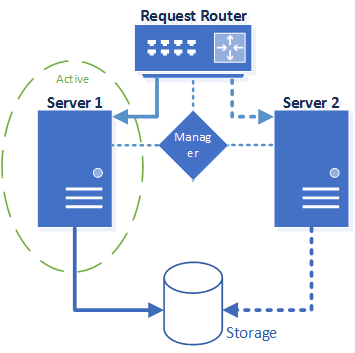
\includegraphics[width=\textwidth/2]{images/ha_cluster_architecture.png}

\textsuperscript{Figure 1.1.1 ``High availability'' cluster architecture}
\end{figure}

Figure 1.1 shows an example architecture of such a ``High availability'' cluster. There are two servers, whereby one server is a replication of the other one. The request router handles the incoming requests and leads them to the active server. If there is a system failure of the active server, the manager will recognize that, and sends a message to the request router to change the request address to the other server. From now on this server will deal with all the requests. Also there is a shared storage for both of the servers in one database. No matter which one is active they can both access this database.\textsuperscript{cmp.\cite{4}}

%https://confluence.atlassian.com/bitbucketserver/high-availability-for-bitbucket-server-776640137.html

But those advantages don't have to stand alone, but they can also be combined, so that you can provide high availability as well as high performance. Because there is an continuously increasing amount of calculations to be made cluster systems are becoming more and more important in modern IT for providing a solution for both problems.

\section{Project objective}
